\documentclass[garamond]{goose-article}

\hypersetup{pdfauthor={T.W.J. de Geus}}

\title{Non-linear elasticity}

\author[1]{Tom de Geus}

%\affil[1]{} % use '\nl' for line-breaks

%\contact{}

%\header{}
%\headerEven{}
%\headerOdd{}

\begin{document}

\maketitle

%\begin{abstract}
%\end{abstract}

%\keywords{}

\section{Consistency check}

To check if the derived tangent $\mathbb{C}$ a \emph{consistency check} can be performed. A (random) perturbation $\delta \bm{\varepsilon}$ is applied. The residual is compared to that predicted by the tangent. For the general case of linearisation, the following holds:
%
\begin{equation}
  \bm{\sigma}\big( \bm{\varepsilon}_\star + \delta \bm{\varepsilon} \big) =
  \bm{\sigma}\big( \bm{\varepsilon}_\star \big) +
  \mathbb{C} \big( \bm{\varepsilon}_\star \big) : \delta \bm{\varepsilon} +
  \mathcal{O}(\delta \bm{\varepsilon}^2)
\end{equation}
%
or
%
\begin{equation}
  \underbrace{
    \bm{\sigma}\big( \bm{\varepsilon}_\star + \delta \bm{\varepsilon} \big) -
    \bm{\sigma}\big( \bm{\varepsilon}_\star \big)
  }_{
    \displaystyle \delta \bm{\sigma}
  } -
  \mathbb{C} \big( \bm{\varepsilon}_\star \big) : \delta \bm{\varepsilon} =
  \mathcal{O}(\delta \bm{\varepsilon}^2)
\end{equation}
%
This allows the introduction of a relative error
%
\begin{equation}
  \eta =
  \Big|\Big|
    \delta \bm{\sigma} -
    \mathbb{C}(\bm{\varepsilon}_\star) : \delta \bm{\varepsilon}
  \Big|\Big|
  /
  \Big|\Big| \delta \bm{\sigma} \Big|\Big|
\end{equation}
%
This \emph{truncation error} thus scales as $\eta \sim || \delta \bm{\varepsilon} ||^2$ as depicted in Figure~\ref{fig:consistency:expected}. As soon as the error becomes sufficiently small the numerical \emph{rounding error} becomes more dominant, the scaling thereof is also included in Figure~\ref{fig:consistency:expected}.

\begin{figure}[htp]
  \centering
  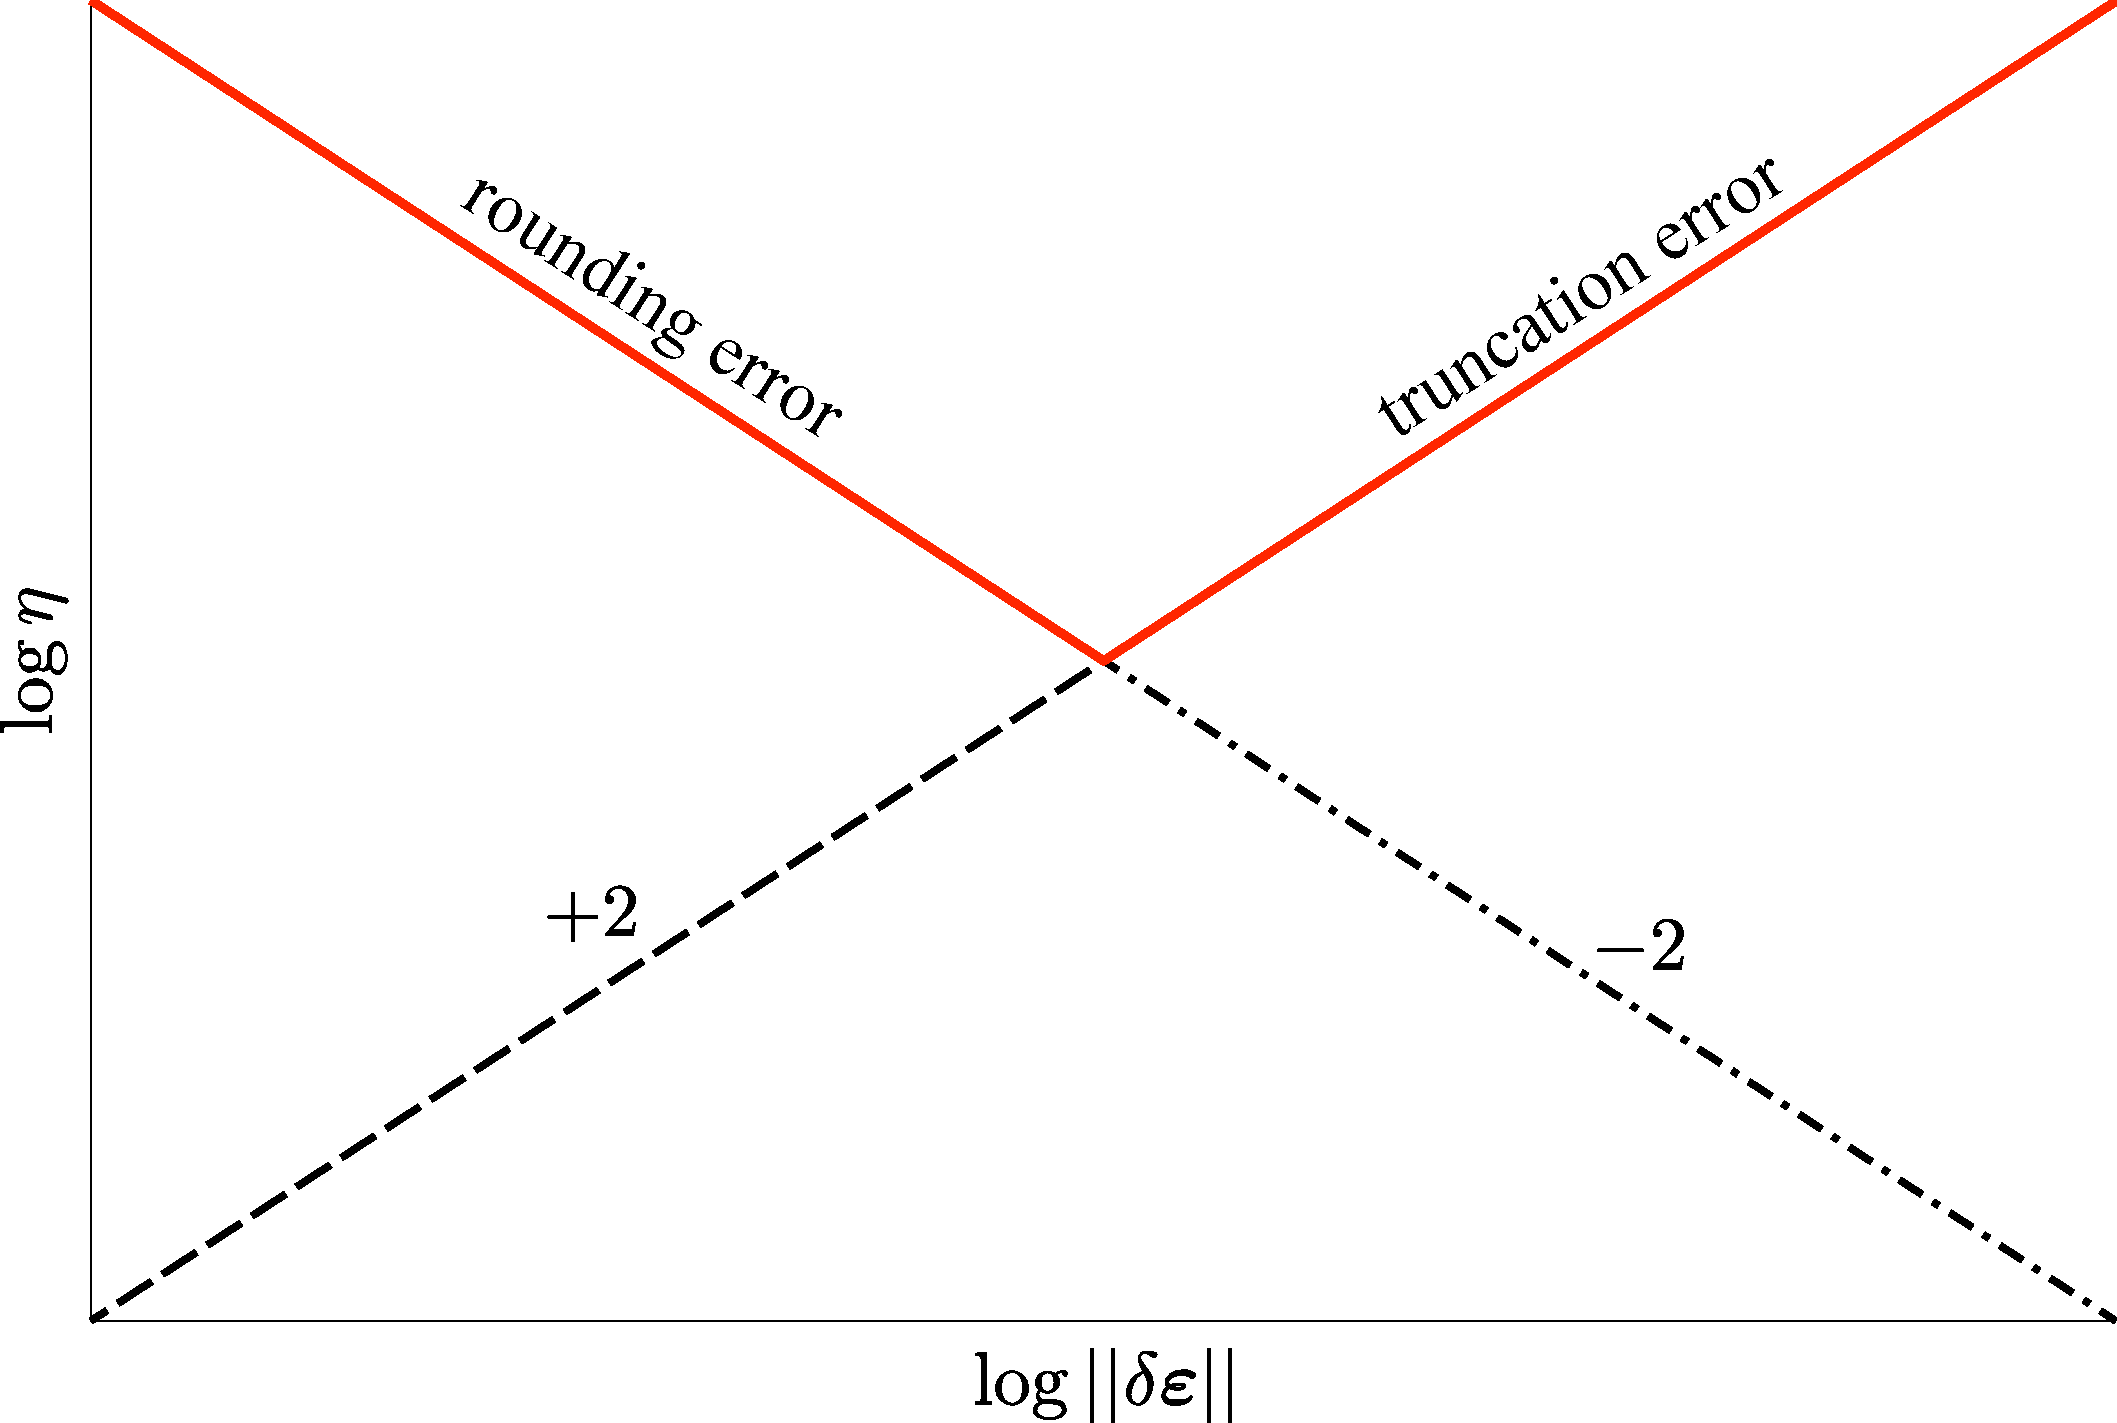
\includegraphics[width=.5\textwidth]{figures/consistency}
  \caption{Expected behaviour of the consistency check, see \citet[p.~9]{Heath2002}.}
  \label{fig:consistency:expected}
\end{figure}

The measurement of $\eta$ and a function of $|| \delta \bm{\varepsilon} ||$, as depicted in Fig.~\ref{fig:consistency}, indeed matches the prediction in Fig.~\ref{fig:consistency:expected}.

\begin{figure}[htp]
  \centering
  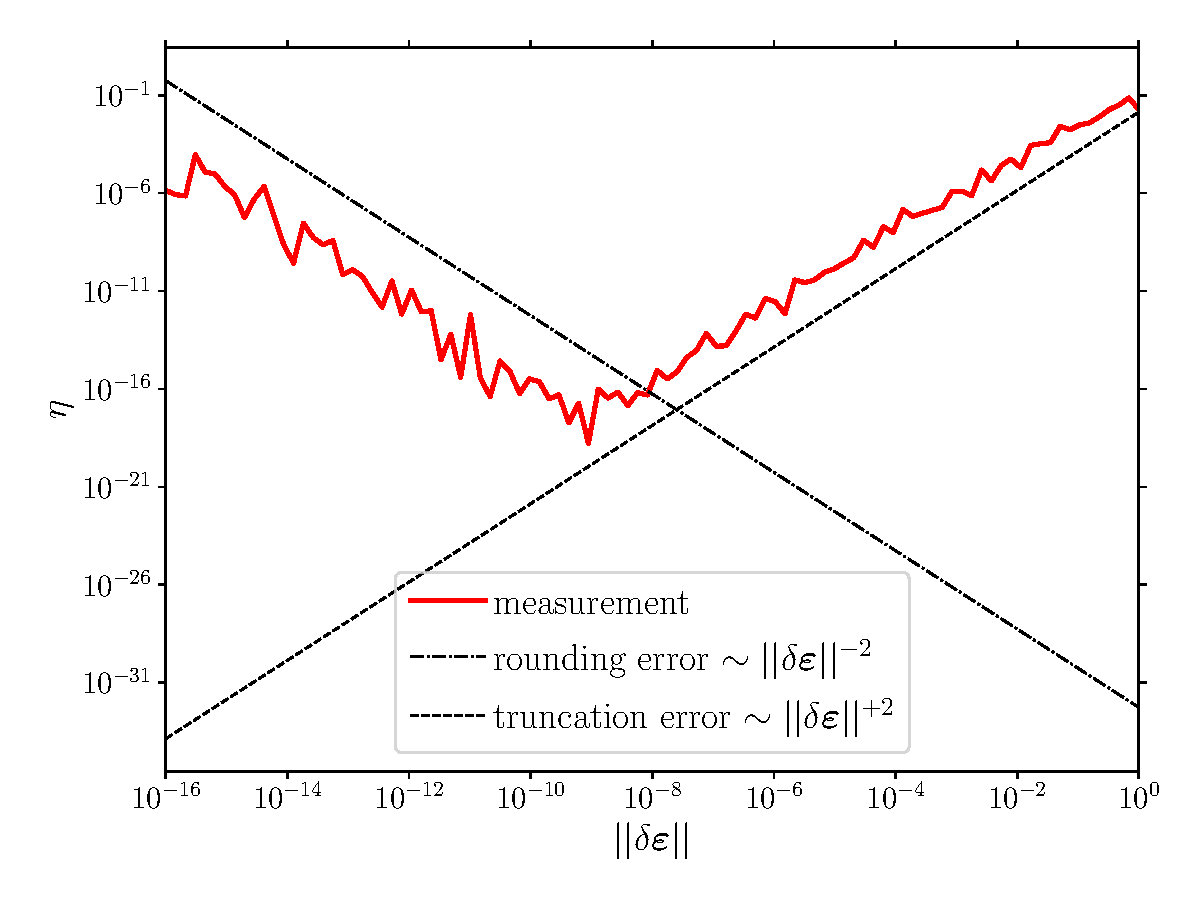
\includegraphics[width=.5\textwidth]{examples/consistency}
  \caption{Measured consistency check, cf.\ Fig.~\ref{fig:consistency:expected}.}
  \label{fig:consistency}
\end{figure}

\bibliography{library}

\end{document}
